\documentclass[14pt]{article}
\usepackage{amsmath}
\usepackage{listings} % For writing code see http://ctan.org/pkg/listings
\usepackage{graphicx}
\usepackage{float}
\usepackage[margin=1.0in]{geometry}
\usepackage{mdframed}
\usepackage{hyperref}

\title{CS665 Final project Spring 2017}
\author{Nicol\'as Garavito-Camargo}
\date{}

\begin{document}
\maketitle

\section*{Introduction and project Goal}

Deriving the gravitational potentials of galaxies is key to
understand the dynamics of this systems. Al galaxy main components
are a stellar disk, a stellar spherical bulge and a spherical Dark Matter halo. The
potential of each component depend on its mass and in their geometry
(in general gravitational potential of symmetric systems are easy to
model). The total galaxy potential is the sum of its components. However,
galaxies are not always isolated, in fact our own galaxy the Milky
Way (MW) is interacting with a smaller galaxy, the Large Magellanic Cloud (LMC).
Due to this interaction, the potential of the Milky Way galaxy is not
only the potential of its components, the LMC have to be also take
into account. The LMC is inducing two major effects. 1) Its mass induce a
gravitational force in the MW as a result the shape of the disk and
the halo is affected. 2) To properly model the gravitational potential
of the MW the potential of the LMC must be included. The former is not 
an easy due to the irregular shape of the LMC.\\

In order to overcome these problems, N-body simulations are a very
common method to properly model interacting galaxies in astronomy. 
N-body simulations model a galaxy as a collection of points and solve
the equations of motions of each point in an iterative scheme: First 
the gravitational potential that each particle feels due to the presence of
the other particles is computed using the gravitational on all the
particles. After the potential of all the particles are
computed the trajectories of this particles can be derived by solving
Newton's equations of motions for each particle for time step $\Delta
t$. Then the potential in the new positions is again computed. This
steps are repeated until the desired time for evolution $t$ is
achieved. This method is particularly useful when the interactions of
galaxies want to be studied.\\

However N-body simulations are computationally expensive and therefore difficult to 
reproduce for the community. A solution to this problem would be to
characterize the potential from the particle distribution in N-body
simulations. This can be done by approximating the underlying
gravitational potential to an analytic function that represents well
enough the global galaxy potential. This analytic function can then be
expanded in a series of orthogonal basis functions, see
\S \ref{sec:methods} for details. In order to find the number of terms
and the amplitude of the expansion terms a set of coefficients have to
be computed using the spatial distribution of particles in the N-body
simulation. However it is unclear how to properly choose the number of
parameters needed that better reproduce the gravitational potential.
\textbf{The goal of this project is to find the best set of coefficients
that best describe the potential of the system.}
This is going to be done by comparing the potential computed with
expansions method to that from the N-body simulation. Then the
difference is going to be minimized as a function of the number of
coefficients.

\section*{Methods}\label{sec:methods}

In order to characterize the gravitational potential of the N-body
simulations from the distribution of particles the following method is
applied.

\begin{enumerate}
\item Assume an underlying form of the potential for spherical
systems.

\item Expand the potential in basis functions.

\item Compute the potential

\item 

\end{enumerate}

\begin{equation}
\Delta \Phi = | \Phi_{analytic} - \Phi_{bfe} |
\end{equation}



\section*{Results \& discussion}



\begin{figure}[H]
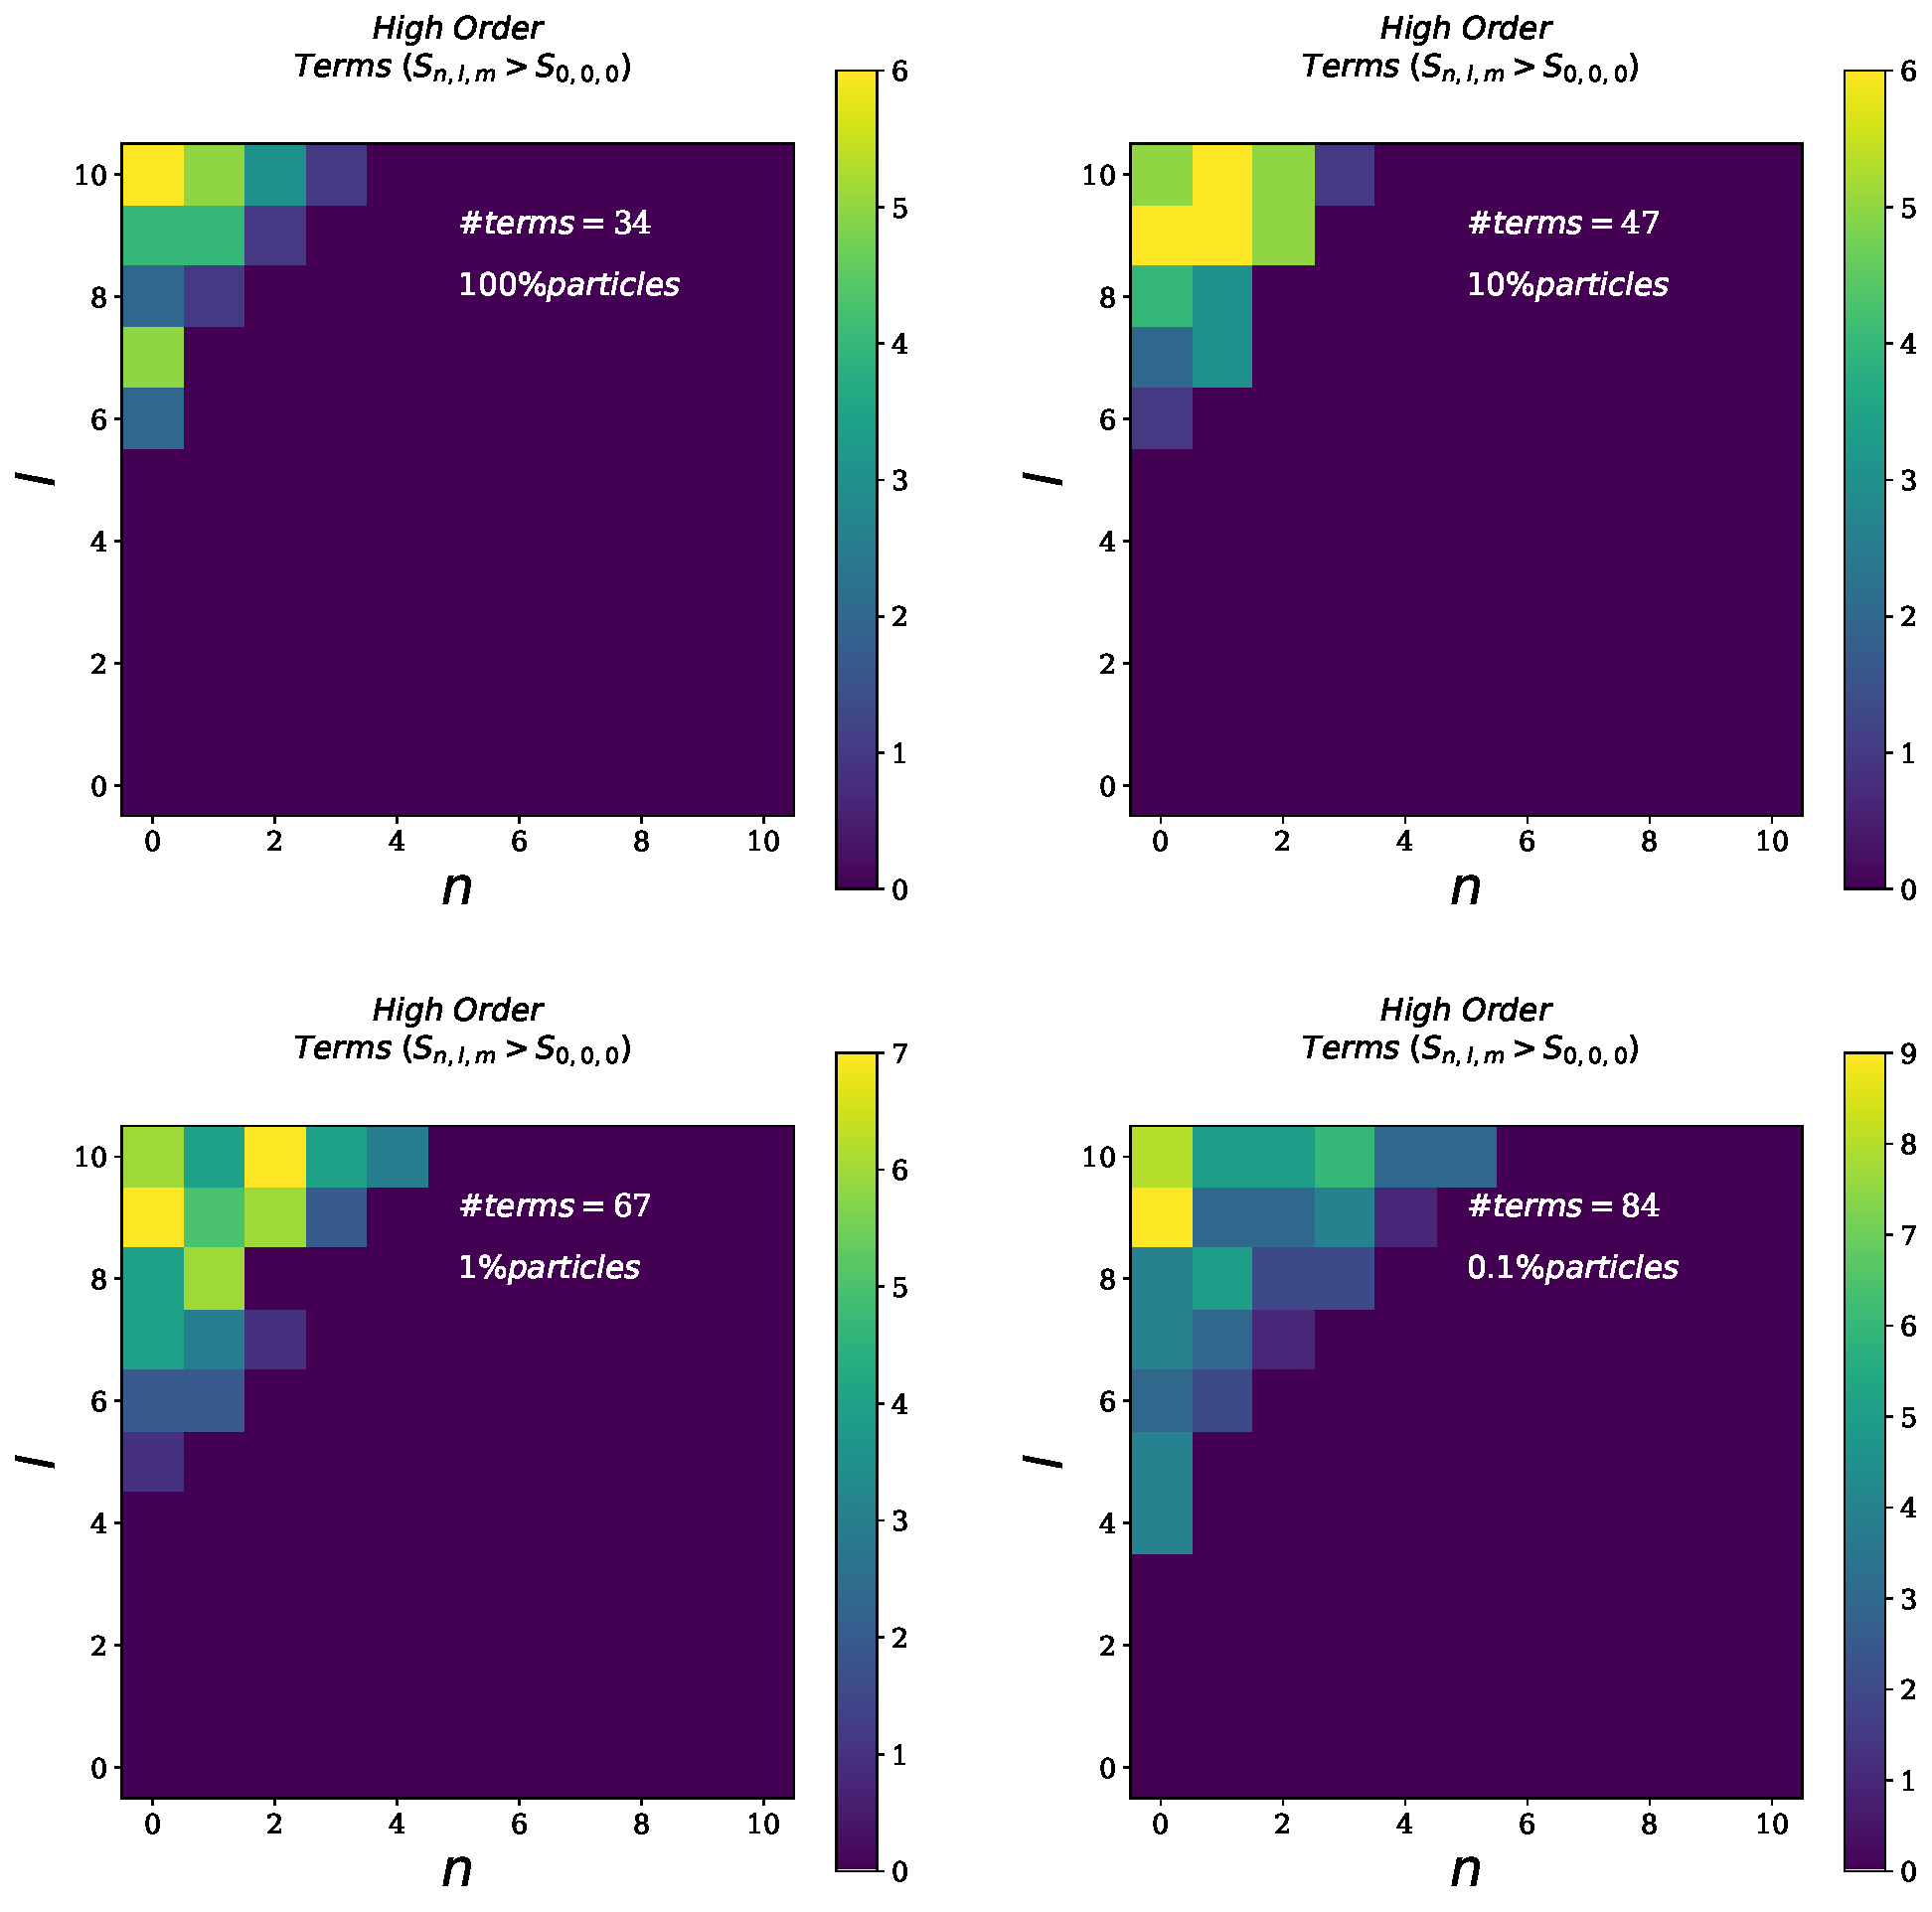
\includegraphics[scale=0.5]{n_terms.pdf}
\end{figure}


\begin{figure}[H]
\centering
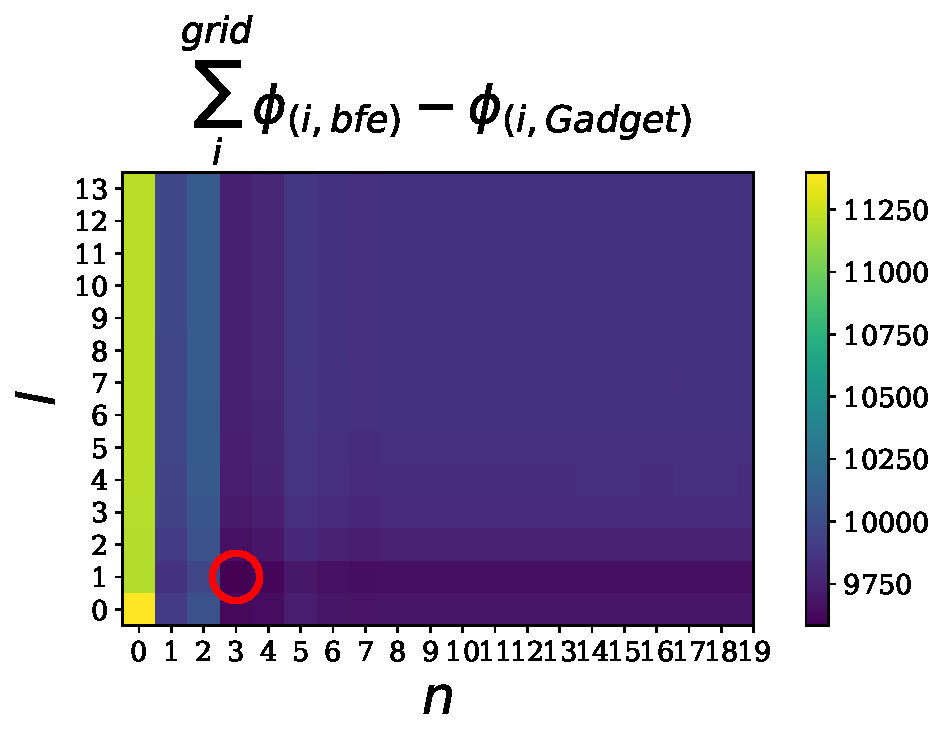
\includegraphics[scale=0.7]{potential_dif_Ncoeff_dep.pdf}
\end{figure}

\section*{Future work:}

Given the analytic difficulty it was hard to convert this problem
into a minimizing problem in which something like.


\end{document}
